\documentclass[border=3pt,tikz]{standalone}

\usepackage{amsmath}
\DeclareMathOperator{\asinh}{asinh}
% taken from
% https://tex.stackexchange.com/questions/153957/drawing-neural-network-with-tikz
\usepackage{tikz}
\usepackage{etoolbox} % for \ifnumcomp
\usepackage{listofitems} % for \readlist to create arrays
\usepackage[T1]{fontenc}
\usetikzlibrary{math} 
\definecolor{myorange}{HTML}{EC6500}
\definecolor{myred}{HTML}{E6001A}
\definecolor{myblue}{HTML}{005AA9}
\definecolor{mygreen}{HTML}{009D81}
\definecolor{mydarkorange}{HTML}{A94913}
\definecolor{mydarkred}{HTML}{961C26}
\definecolor{mydarkblue}{HTML}{243572}
\definecolor{mydarkgreen}{HTML}{00715E}
\tikzset{>=latex} % for LaTeX arrow head
%\colorlet{myred}{red!80!black}
%\colorlet{myblue}{blue!80!black}
%\colorlet{mygreen}{green!60!black}
%\colorlet{mydarkred}{myred!40!black}
%\colorlet{mydarkblue}{myblue!40!black}
%\colorlet{mydarkgreen}{mygreen!40!black}
\tikzstyle{node}=[very thick,circle,draw=myblue,minimum size=22,inner sep=0.5,outer sep=0.6]
\tikzstyle{connect}=[->,thick,black,shorten >=1]
\tikzset{ % node styles, numbered for easy mapping with \nstyle
	node 1/.style={node,black,draw=white},
	node 2/.style={node,black,draw=black,fill=black!20},
	node 3/.style={node,mydarkblue,draw=myblue,fill=myblue!20},
	node 4/.style={node,mydarkorange,draw=myorange,fill=myorange!20},
	node 5/.style={node,mydarkred,draw=myred,fill=myred!20},
}
\def\nstyle{int(\lay<\Nnodlen-1?min(3,\lay):(\lay==\Nnodlen-1?4:5))} % map layer number onto 1, 2, 3, or 4

\usepackage{helvet}
\usepackage[outline]{contour}
\contourlength{3.0pt}

\begin{document}
	
	
	% NEURAL NETWORK
	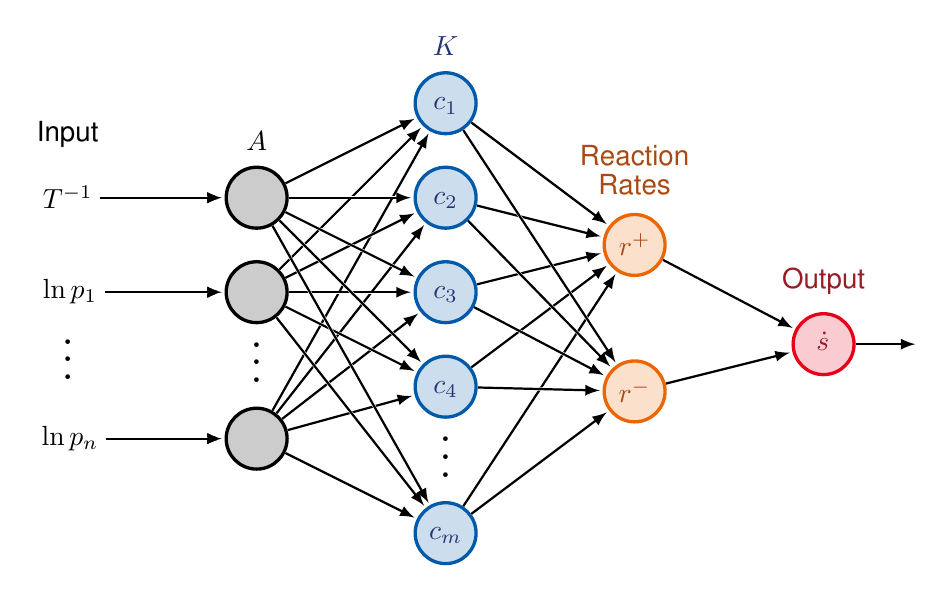
\begin{tikzpicture}[x=2.4cm,y=1.2cm]
		\readlist\Nnod{3,3,5,2,1} % array of number of nodes per layer
		\readlist\Nstr{n,n+1,m,2,} % array of string number of nodes per layer
		\readlist\Cstr{\ln p,,c,$$r$$,$$\dot{s}$$} % array of coefficient symbol per layer
%		\readlist\Cstr{p,\ln p,,,,$$\dot{s}$$}
		\def\yshift{0.55} % shift last node for dots
		
		% LOOP over LAYERS
		\foreachitem \N \in \Nnod{
			\def\lay{\Ncnt} % alias of index of current layer
			\pgfmathsetmacro\prev{int(\Ncnt-1)} % number of previous layer
			\foreach \i [evaluate={\c=int(\i==\N); \y=\N/2-\i-\c*\yshift;
				\x=\lay; \n=\nstyle;
				\index=(\i<\N?int(\i):"\Nstr[\n]");
				\indexshifted=(\i<\N?int(\i-1):"\Nstr[\n]");}] in {1,...,\N}{ % loop over nodes
				% NODES
				% -----
				
				% layer 1 is special
				\ifnum \lay=1
					\ifnum \i=1
						\node[node \n] (N\lay-\i) at (\x,\y) {$T^{-1}$};
					\else
						\node[node \n] (N\lay-\i) at (\x,\y) {$\strut\Cstr[\n]_{\indexshifted}$};
					\fi
				\fi
				% layer 2 is not labeled
				\ifnum \lay=2
					\node[node \n] (N\lay-\i) at (\x,\y) {};
				\fi
							
				
				\ifnum \lay=4
					\ifnum \i=1
						\node[node \n] (N\lay-\i) at (\x,\y) {$r^+$};
					\fi
					\ifnum \i=2
						\node[node \n] (N\lay-\i) at (\x,\y) {$r^-$};
					\fi
				\else
					% all other layers are ordinarily labeled
					\ifnum \lay>2
						\node[node \n] (N\lay-\i) at (\x,\y) {$\strut\Cstr[\n]_{\index}$};
					\fi
				\fi
				
				
				
				% CONNECTIONS
				\ifnumcomp{\lay}{>}{2}{ % connect to previous layer
					\foreach \j in {1,...,\Nnod[\prev]}{ % loop over nodes in previous layer
						\draw[white,line width=1.2,shorten >=1] (N\prev-\j) -- (N\lay-\i);
						\draw[connect] (N\prev-\j) -- (N\lay-\i);
					}
					\ifnum \lay=\Nnodlen
					\draw[connect] (N\lay-\i) --++ (0.5,0); % arrows out
					\fi
				}{
				
					\ifnumcomp{\lay}{>}{1}{ % connect to previous layer
						\foreach \j in {1,...,\Nnod[\prev]}{ % loop over nodes in previous layer
							\draw[white,line width=1.2,shorten >=1] (N\prev-\i) -- (N\lay-\i);
							\draw[connect] (N\prev-\i) -- (N\lay-\i);
						}
					}
					{}%{\draw[connect] (0.5,\y) -- (N\lay-\i);} % arrows into first layer
				}
				
			}
			\ifnumcomp{\N}{<}{3}{} % no dots
			\path (N\lay-\N) --++ (0,1+\yshift) node[midway,scale=1.6] {$\vdots$}; % dots
		}
		
		% LABELS
		\node[above=3,align=center,black,font=\fontfamily{phv}\selectfont] at (N1-1.90) 
		{Input};
%		\node[above=2,align=center,black] at (5.5,-1.125) 
%		{$z\cdot\sinh(y)$};
		\node[above=2,align=center,black,font=\fontfamily{phv}\selectfont] at (N2-1.90) 
		{$A$};
%		\node[above=2,align=center,black,font=\fontfamily{phv}\selectfont] at (N3-1.90) 
%		{Minmax\\[-0.2em]Mapped};
		\node[above=2,align=center,mydarkblue,font=\fontfamily{phv}\selectfont] at (N3-1.90) 
		{$K$};
		\node[above=3,align=center,mydarkorange,font=\fontfamily{phv}\selectfont] at (N4-1.90) 
		{\contour{white} {\shortstack{Reaction\\ Rates}}};
		\node[above=3,align=center,mydarkred,font=\fontfamily{phv}\selectfont] at (N\Nnodlen-1.90) 
		{Output};
%		\node[above=0,align=center,font=\fontfamily{phv}\selectfont] at (N\Nnodlen-1.90) {\contour{white} {sinh(y)}};
		
	\end{tikzpicture}
	
	
\end{document}